%*****************************************
\chapter{The $\lambda$-calculus}\label{ch:lambda}
%*****************************************
\section{History and overview}
\section{The Abstract Setting: Rewriting Theory}
The $\lambda$-calculus is essentially a rewrite system. Thus, before introducing it, we present some fundamentals of rewriting theory. This way we can insert the $\lambda$-calculus in a more general setting, allowing a deeper and often simpler analysis. Rewriting is crucial in computer science since basically any computation can be seen as a process of rewriting. In fact, digital computers work through formal manipulation of symbols, in a purely syntactic way. Rewriting theory was born together with logic, but now it has an independent status, as shown by the annual International Conference on Rewriting Techniques and Applications (RTA) \cite{noauthor_rta_nodate}, now part of the International Conference on Formal Structures for Computation and Deduction along with the  International Conference on Typed Lambda Calculi and Applications \cite{noauthor_notitle_nodate}, just to remark the strong connection between the two fields. The basic object of investigation of rewriting theory is the abstract reduction (or rewrite) system. 

\begin{definition}
	An \emph{abstract reduction system} (ARS) is a pair $(A,\rightarrow)$ where $A$ is a set with cardinality at most countable and $\rightarrow\,\subseteq A\times A$.
\end{definition}
$A$ is the set of \emph{terms} and $\rightarrow$ is the \emph{reduction relation}. If $(a,b)\in\,\rightarrow$ for $a,b\in A$, we write $a\rightarrow b$ and intuitively this means that ``$a$ can be rewritten in $b$''. $\twoheadrightarrow$ is the reflexive and transitive closure of $\rightarrow$. A \emph{reduction sequence} is a finite or infinite sequence $\sigma:a_0\rightarrow a_1\rightarrow\cdots$. If $\sigma$ is finite $|\sigma|$ is the \emph{length} of $\sigma$. Since rewriting is a model of computation, we are interested in defining termination. We say that $a\in A$ is in \emph{normal form} if there exist no $b\in A$ such that $a\rightarrow b$. We call $\mathbf{NF}(A)$ the set of terms in normal form of $A$. A term $a$ is \emph{(weakly) normalising} if there exists a reduction sequence such that $a\twoheadrightarrow b$ and $b$ is in normal form. A term $a$ is \emph{strongly normalising} if every reduction sequence from $a$ is finite.  A lot of interesting properties can be defined for ARSs. The interested reader can refer to the two main monographs on the subject \cite{terese_term_2003,baader_term_1999} for a complete account on them. However, it is worth mentioning here a very important property, confluence.
\begin{definition}
	Let $(A,\rightarrow)$ be an ARS. $\rightarrow$ is \emph{confluent} or \emph{Church-Rosser} (CR), if for each $a\in A$ such that $a\twoheadrightarrow b$ and $a\twoheadrightarrow c$, there exists $d\in A$ such that $b\twoheadrightarrow d$ and $c\twoheadrightarrow d$.
\end{definition}
Confluence is a desirable property because intuitively it states that no matter the reduction path followed, one can always reach the very same term, possibly going further with the reductions (Figure \ref{figure:confluence}). In particular confluence is sufficient for an ARS to satisfy the unique normal form property, we are defining below.
\begin{figure}
	\centering
	\subfloat[]{{	
			\begin{tikzpicture}
			[node distance=20mm, auto, transform shape]
			\node (m) at (0,0) {$a$};
			\node (n) at (-1,-1) {$b$};
			\node (l) at (1,-1) {$c$};
			\draw (m) edge[->>] node[left=5pt] {} (n);
			\draw (m) edge[->>] node[right=5pt] {} (l);
			\end{tikzpicture}}}
	\qquad
	\subfloat[]{{	
			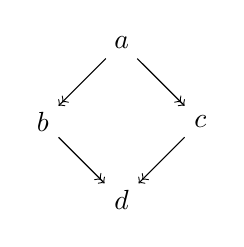
\begin{tikzpicture}
			[node distance=20mm, auto, transform shape]
			\node (m) at (0,0) {$a$};
			\node (n) at (-1,-1) {$b$};
			\node (l) at (1,-1) {$c$};
			\node (p) at (0,-2) {$d$};
			\draw (m) edge[->>] node[left=5pt] {} (n);
			\draw (m) edge[->>] node[right=5pt] {} (l);
			\draw (n) edge[->>] node[left=5pt] {} (p);
			\draw (l) edge[->>] node[right=5pt] {} (p);
			\end{tikzpicture}}}
	\caption{CR holds if (a) implies (b)}
	\label{figure:confluence}
\end{figure}
\begin{definition}
	Let $(A,\rightarrow)$ be an ARS. $\rightarrow$ has the \emph{unique normal form property} (UN) if for each $a,b,c\in A$, such that $a\twoheadrightarrow b$, $a\twoheadrightarrow c$, and $b,c\in\mathbf{NF}(A)$, then $b\equiv c$.
\end{definition}
Uniqueness of normal form is a key aspect when we are dealing with ARSs. In fact, typically, we want that a given term always terminates in the same result, although possibly following different paths.
\begin{proposition}
	Let $(A,\rightarrow)$ be an ARS. If $\rightarrow$ is confluent then $\rightarrow$ has the unique normal form property.
\end{proposition}
\begin{proof}
	By contradiction, let us consider an ARS $(A,\rightarrow)$ such that $\rightarrow$ is confluent but does not satisfy UN. Then there exist $a,b,c\in A$, such that $a\twoheadrightarrow b$, $a\twoheadrightarrow c$, $b,c\in\mathbf{NF}(A)$ and $b\not\equiv c$. Since $\rightarrow$ is confluent, there exists $d\in A$ such that $b\twoheadrightarrow d$ and $c\twoheadrightarrow d$. Since both $b$ and $c$ are in normal form this would imply $d\equiv b\equiv c$ but this is impossible since $b$ and $c$ are different normal forms.
\end{proof}
ARSs are sets endowed with a relation, and are thus
inherently nondeterministic, if we consider rewriting as a model of a computation. The notion of reduction strategy allows us to turn reduction into a deterministic process.
\begin{definition}[Deterministic Strategies]\label{def:determstrat}
	Given an ARS $(A,\rightarrow)$, a \emph{deterministic reduction
		strategy for $A$} is a partial function $\mathsf{S}:A\rightharpoonup A$
	such that $\mathsf{S}(a)$ is defined if and only if $a$ is not in
	normal form and $a\rightarrow\mathsf{S}(a)$ whenever $\mathsf{S}(a)$
	is defined.
	%$\mathsf{S}(a)\in\{b\,|\,a\rightarrow b\}$.
\end{definition}
If $\sigma:a_0\rightarrow a_1\rightarrow\cdots\rightarrow a_n$ is a
reduction sequence under strategy $\mathsf{S}$ and $a_n$ is in normal
form, we write $\nsteps{\mathsf{S}}(a_0)=n=|\sigma|$. If
$\sigma:a_0\rightarrow a_1\rightarrow\cdots$ is infinite, we say that
$\nsteps{\mathsf{S}}(a_0)=+\infty$. A strategy $\mathsf{S}$ is \emph{normalising} if for each weakly normalising term $a$, $\nsteps{\mathsf{S}}(a)<+\infty$. Reductions to normal form of the same term under different strategies can be of different lengths, and in particular some of them can be infinite. However, under particular conditions, all strategies are equivalent.
\begin{definition}
	An ARS $(A,\red)$ satisfies the \emph{(weak) diamond property} (WDP) if and only if for each term $a\in A$, if $a\red b$ and $a\red c$ with $b\neq c$, then there exists a term $d\in A$ such that $b\red d$ and $c\red d$. 
\end{definition}
Intuitively an ARS satisfies the WDP if we can close every diagram in one step, forming a diamond (Figure \ref{figure:diam}). This very strong property is sufficient to state that all reduction sequences from a term to its normal form have the \emph{same} length, i.e. no matter the strategy chosen to select the reduct.
\begin{figure}
	\centering
	\subfloat[]{{	
			\begin{tikzpicture}
			[node distance=20mm, auto, transform shape]
			\node (m) at (0,0) {$a$};
			\node (n) at (-1,-1) {$b$};
			\node (l) at (1,-1) {$c$};
			\node (eq) at (0,-1) {$\neq$};
			\draw (m) edge[->] node[left=5pt] {} (n);
			\draw (m) edge[->] node[right=5pt] {} (l);
			\end{tikzpicture}}}
	\qquad
	\subfloat[]{{	
			\begin{tikzpicture}
			[node distance=20mm, auto, transform shape]
			\node (m) at (0,0) {$a$};
			\node (n) at (-1,-1) {$b$};
			\node (l) at (1,-1) {$c$};
			\node (p) at (0,-2) {$d$};
			\draw (m) edge[->] node[left=5pt] {} (n);
			\draw (m) edge[->] node[right=5pt] {} (l);
			\draw (n) edge[->] node[left=5pt] {} (p);
			\draw (l) edge[->] node[right=5pt] {} (p);
			\end{tikzpicture}}}
	\caption{WDP holds if (a) implies (b)}
	\label{figure:diam}
\end{figure}
\begin{lemma}[]\label{lemma:weak}
	If an ARS $(A,\red)$ satisfies the weak diamond property, then for each term $a\in A$ that has a normal form all reduction sequences from $a$ to its normal form have the same length.
\end{lemma}
\begin{proof}
	The proof by induction is given with all details in \cite{lago_invariant_2005}.
\end{proof}
\section{The Syntax}
We now define a specific ARS, the $\lambda$-calculus. We start defining the set of its terms. As usual in theoretical computer science terms are inductively defined by a context-free grammar \cite{backus_syntax_1959}.
\begin{definition}
	Assume a countable infinite set $\mathcal{V}$ of variables. The
	$\lambda$-\emph{calculus} is the language of terms defined by
	the following grammar:
	$$
	\termone,\termtwo\bnf\varone\in\mathcal{V}\midd\termone\termtwo\midd\abstr{\varone}{\termone}
	$$
	We denote by $\Lambda$ the set of all $\lambda$-terms.
\end{definition}
Since $\lambda$-terms are defined inductively from other $\lambda$-terms via application and abstraction, it is natural to define a function that maps each term to the set of its subterms. We will often use a pattern-matching-like syntax to define properties of $\lambda$-terms. In this case the match is against the rule of the grammar used to form the term (akin to sum types in functional programming languages).
\begin{THESIS}
	\begin{definition}
		The set of \emph{subterms} $\mathsf{Sub(\mathit{\termone})}$ of a term $\termone$ is defined inductively on the structure of $\termone$ as follows.
		\begin{align*}
		&\mathsf{Sub(\mathit{x})}=\{x\},\\
		&\mathsf{Sub(\mathit{\termtwo\termthree})}=\mathsf{Sub(\mathit{\termtwo})}\cup \mathsf{Sub(\mathit{\termthree})}\cup\{\termtwo\termthree\},\\
		&\mathsf{Sub(\mathit{\lambda x.\termtwo})}=\mathsf{Sub(\mathit{\termtwo})}\cup \{\lambda x.\termtwo\}.
		\end{align*}
	\end{definition}
\end{THESIS}
\begin{THESIS}
	The concept of bound and free variables is ubiquitous in logic. Informally, names of bounded occurrences of variables are meaningless, in the sense that they can be renamed without changing the semantics of a term, provided that new names are \emph{fresh}, i.e. they do not occur anywhere in the term. This observation leads to the definition of $\alpha$-conversion.
	\begin{definition}
		A variable $x$ occurs \emph{bound} in $\termone$, if $\lambda x.\termtwo\in\mathsf{Sub(\mathit{\termone})}$ for some term $\termtwo$. The set of \emph{free variables} $FV(\termone)$ of a term $\termone$ is defined inductively on the structure of $\termone$ as follows.
		\begin{align*}
		&FV(x)=\{x\},\\
		&FV(\termtwo\termthree)=FV(\termtwo)\cup FV(\termthree),\\
		&FV(\lambda x.\termtwo)=FV(\termtwo)\setminus\{x\}.
		\end{align*}
	\end{definition}
	\begin{definition}
		Two terms $\termone$ and $\termtwo$ are said to be \emph{$\alpha$-convertible} if one can derive the same term from both purely by renaming bound occurrences of variables to fresh variables.
	\end{definition}
	Since $\alpha$-conversion is an equivalence relation, from now on we consider $\lambda$-terms modulo $\alpha$-equivalence. Indeed if two terms $\termone$ and $\termtwo$ are $\alpha$-convertible we consider them equivalent at syntactic level and we write $\termone\equiv\termtwo$. Moreover it is worth mentioning that there exist different representations of $\lambda$-terms in which there are not bound variables at all. The most famous is the use of De Brujin indexes, used in most compilers and interpreters of functional programming languages \cite{de_bruijn_lambda_1972}.
	
\end{THESIS}
\begin{THESIS}
	In order to define $\beta$-reduction, the reduction relation of the $\lambda$-calculus, we need to formally define the concept of substitution. 
	We assume from now the \emph{Barendregt's variable convention} for which every term has all bound variables distinct from each other and from any free variable. This can be done since we are considering terms modulo $\alpha$-equivalence.
	\begin{definition}
		We denote by $\termone\{\termtwo/x\}$ the \emph{(capture-avoiding) substitution} of variable $x$ by term $\termtwo$ in term $\termone$ performed in the following way.
		\begin{align*}
		&x\{\termtwo/x\}=\termtwo,\\
		&y\{\termtwo/x\}=y\qquad\textrm{if $x\not\equiv y$},\\
		&(\termone\termthree)\{\termtwo/x\}=(\termone\{\termtwo/x\}\termthree\{\termtwo/x\}),\\
		&(\lambda y.\termone)\{\termtwo/x\}=(\lambda y.\termone\{\termtwo/x\}).
		\end{align*}
	\end{definition}
	The following Lemma asserts formally commutativity of substitutions.
	\begin{lemma}[Substitution Lemma]
		For any $\termone,\termtwo,\termthree\in\Lambda$ if $x\neq y$ and $x\not\in FV(\termthree)$, then
		$$
		\termone\{\termtwo/x\}\{\termthree/y\}\equiv\termone\{\termthree/y\}\{\termtwo\{\termthree/y\}/x\}.
		$$
	\end{lemma}
\end{THESIS}
Reduction will be defined based on the notion of a context, which
needs to be given a formal status.
\begin{definition}
	We define (one-hole) \emph{contexts} by the following grammar:
	$$
	\contone,\conttwo\bnf\Box\midd\contone\termone\midd\termone\contone\midd\abstr{\varone}{\contone}
	$$
	We denote with $\Lambda_\Box$ the set of all contexts.
\end{definition}
Intuitively, contexts are $\lambda$-terms with a hole that can be
filled with another $\lambda$-term. We indicate with
$\contone[\termone]$ the term obtained by replacing $\Box$ with
$\termone$ in $\contone$. Those $\lambda$-terms in the form
$\rdxone=(\lambda x.\termone)\termtwo$ are called \emph{$\beta$-reducible expressions} or
$\beta$-\emph{redexes} and $\termone\{\termtwo/x\}$ is said to be
the \emph{contractum} of $\rdxone$. This is justified by the following definition.
\begin{definition}
	The relation of $\beta$-\emph{reduction}, $\redbeta\subseteq\Lambda\times\Lambda$, is defined as
	$$
	\redbeta = \{(\contone[(\lambda x.\termone)\termtwo],\, \contone[\termone\{\termtwo/x\}])\, |\, \termone, \termtwo\in\Lambda, \contone\in\Lambda_\Box\}.
	$$
\end{definition}
This way we have defined the $\lambda$-calculus as the ARS $(\Lambda,\redbeta)$. We denote by $\Lambda_\mathsf{WN}$ the set of weakly normalising terms of $\Lambda$. In the following sections a restriction of the $\beta$-reduction will be useful.
\begin{definition}
	The relation of $\mathsf{ANF}$-$\beta$-\emph{reduction}, $\redbetaanf\subseteq\Lambda\times\Lambda$, is defined as
	$$
	\redbetaanf = \{(\contone[(\lambda x.\termone)\termtwo],\, \contone[\termone\{\termtwo/x\}])\, |\, \termone, \termtwo\in\Lambda,\,\termtwo\in\textbf{NF}(\Lambda),\, \contone\in\Lambda_\Box\}.
	$$
\end{definition}
\subsection{Two Subcalculi of $\Lambda$}
%%%%%%%%%%%%%%%%%%%%%%%%%%%%%%%%%%%%%%%%
Full $\lambda$-calculus is very powerful and flexible but it is very hard to study in its full generality. Sometimes it is useful to restrict ourselves to a subset of terms. In particular we focus our attention on two subsystems where terms satisfy a predicate on the number of occurrences of free variables. These systems are meaningful because they are \emph{stable} w.r.t. $\beta$-reduction i.e. if $\termone\in S$ and $\termone\redbeta\termtwo$ then $\termtwo\in S$. A comprehensive treatment is in \cite{sinot_sub-$lambda$-calculi_2008}.
%%%%%%%%%%%%%%%%%%%%%%%%%%%%%%%%%%%%%
\subsubsection{The $\lambda I$-calculus.}
%%%%%%%%%%%%%%%%%%%%%%%%%%%%%%%%%%%%%
The $\lambda I$-calculus was the original calculus studied by Alonzo
Church in the '30 \cite{church_unsolvable_1936}, while
\cite{barendregt_lambda_1984} contains a whole section dedicated to
it. In $\lambda I$-calculus there is no \emph{cancellation}, in that
variables have to occur free \emph{at least once} when forming
abstractions. Terms of the $\lambda I$-calculus are not strongly
normalising in general. As an example, $\bm{\Omega}$ is a $\lambda I$-term.
One can prove, however, the following important result.
\begin{theorem}
	For each term $\termone\in\Lambda_I$, if $\termone$ is weakly normalising, then it is strongly normalising.
\end{theorem}
In other words, all strategies are qualitatively equivalent. This does \emph{not} mean, however, that they are quantitatively equivalent.
%%%%%%%%%%%%%%%%%%%%%%%%%%%%%%%%%%%%%
\subsubsection{The $\lambda A$-calculus.}
%%%%%%%%%%%%%%%%%%%%%%%%%%%%%%%%%%%%%
The $\lambda A$-calculus is the dual of $\lambda I$-calculus and it is
sometimes called \emph{affine} $\lambda$-calculus in the
literature. It is a very weak calculus in which variables bound by
abstractions occur \emph{at most once} free in the abstraction's body,
thus forbidding \emph{duplication}. The $\lambda A$-calculus is strongly
normalising, in a very strong sense: every reduction sequence from a term
$\termone$ has length bounded by the size of $\termone$.
\section{Fundamental Meta-Theory}
In this section we report some fundamental results in the meta-theory of the $\lambda$-calculus.
\begin{theorem}
	The relation $\redbeta$ on $\Lambda$ is confluent.
\end{theorem}
\begin{corollary}
	Let $\termone\in\Lambda$ be a $\lambda$-term. If $\termone\redbeta\termtwo$ and $\termone\redbeta\termthree$, where $\termtwo,\termthree\in\textbf{NF}(\Lambda)$, then $\termtwo\equiv\termthree$.
\end{corollary}
\subsection{Expressiveness}
The $\lambda$-calculus, as we have defined it, in the previous section, turns out to be a Turing-complete formalism. This means that we should be able to use it as a programming language. We are not going to discuss in detail all the encodings, we just limit to a few illuminating examples. For a complete treatment, the interested reader can refer to \cite{barendregt_lambda_1984}.
\paragraph{Integers}
Integer numbers can be encoded as $\lambda$ terms in the following way. They are named Church numerals because this was the original encoding provided by Church.
\begin{itemize}
	\item $\lceil zero\rceil=\lambda f.\lambda x.x$
	\item $\lceil one\rceil=\lambda f.\lambda x.(fx)$
	\item $\lceil two\rceil=\lambda f.\lambda x.(f(fx))$
	\item $\lceil n\rceil=\lambda f.\lambda x.(f^nx)$
\end{itemize}
where $f^nx$ is inductively defined by
$$
f^0x=x\,,\qquad f^kx=f(f^{k-1}x)\,.
$$
\paragraph{Arithmetics}
Once defined numerals, one wants to use them. We give here combinators for addition, multiplication and exponentiation:
\begin{itemize}
	\item $\mathbf{A}=\lambda x.\lambda y.\lambda p.\lambda q.(xp(ypq))$,
	\item $\mathbf{M}=\lambda x.\lambda y.\lambda z.(x(yz))$,
	\item $\mathbf{E}=\lambda x.\lambda y.yx$.
\end{itemize}
\begin{proposition}
	$\mathbf{A}$, $\mathbf{M}$ and $\mathbf{E}$ perform, respectively, addition, multiplication and exponentiation when applied to Church numerals, i.e.
	\begin{itemize}
		\item $\mathbf{A}\lceil n\rceil\lceil m\rceil=\lceil n+m\rceil$,
		\item $\mathbf{M}\lceil n\rceil\lceil m\rceil=\lceil n*m\rceil$,
		\item $\mathbf{E}\lceil n\rceil\lceil m\rceil=\lceil n^m\rceil$, except for $m=0$.
	\end{itemize}
\end{proposition}
The reader can note how easy the whole process is w.r.t other Turing-complete formalisms, such as Turing machines. Sketching a single-tape Turing machine performing multiplication would not be in fact an easy task at all. Besides basic arithmetical operations one could show how to encode all partial recursive functions. In fact it is possible  to encode in the $\lambda$-calculus the so-called initial functions, together with composition, projection, minimisation and primitive recursion operators.
\begin{theorem}
	A function is $\lambda$-definable if and only if it is partial recursive.
\end{theorem}
Actually, one does not need full $\lambda$-calculus to have a Turing-complete language, because also the $\lambda I$-calculus has the same characteristic.
\section{Strategies}
We have already defined what a reduction strategy is, in the abstract. Now we are going to report some results regarding some concrete strategies for the $\lambda$-calculus. Typically, strategies are defined giving the position of the redex to be reduced. Different strategies can lead to completely different reduction sequences and thus to completely different computations. Some, for example, can be non-terminating, while others can terminate in just one step, though starting from the same term. Investigation of reduction strategies is an active field in the programming language community because of the great impact they have on performances. We start defining two classical strategies.
\begin{definition}
	\emph{Leftmost-outermost} $(\pslo)$ is a deterministic reduction
	strategy in which $\pslo(\termone)=\termtwo$ if and only if
	$\termone\redbeta\termtwo$ and the redex contracted in $\termone$ is
	the \emph{leftmost} among the ones in $\termone$ (measuring the
	position of a redex by its beginning). If $\pslo(\termone)=\termtwo$,
	we write $\termone\redlo\termtwo$.
\end{definition}
\begin{definition}
	\emph{Rightmost-innermost} $(\psri)$ is a deterministic reduction
	strategy in which $\psri(\termone)=\termtwo$ if and only if
	$\termone\redbeta\termtwo$ and the redex contracted in $\termone$ is
	the \emph{rightmost} among the ones in $\termone$ (measuring the
	position of a redex by its beginning). Again, if
	$\psri(\termone)=\termtwo$, we write $\termtwo\redri\termtwo$.
\end{definition}
\begin{example}\label{example:canc}
	Let $\bm{\omega}=\lambda x.xx$ and
	$\bm{\Omega}=\bm{\omega\omega}$. We now consider the reduction of
	the term $(\lambda x.y)\bm{\Omega}$ according to leftmost-outermost and
	rightmost-innermost stratgies.
	\begin{align*}
		(\lambda x.y)\bm{\Omega}&\redlo y\\
		(\lambda x.y)\bm{\Omega}&\redri(\lambda x.y)\bm{\Omega}\redri(\lambda x.y)\bm{\Omega}\redri\cdots
	\end{align*}
	The term $\bm{\Omega}$ is a looping combinator i.e. it reduces to
	itself. However, in $(\lambda x.y)\bm{\Omega}$ the argument
	$\bm{\Omega}$ is discarded since the function returns the constant
	$y$. Thus leftmost-outermost (akin to call-by-name in functional
	programming languages) yields a normal form in one step. Conversely,
	rightmost-innermost (akin to call-by-value) continues to evaluate
	the argument $(\lambda x.y)\bm{\Omega}$, though it is useless, and
	rewrites always the same term, yielding to a non-terminating
	process.
\end{example}
\begin{example}\label{example:copy}
	Let $\bm{I}=\lambda x.x$. We now consider the reduction of the term
	$(\lambda x.xx)(\bm{II})$, according to $\pslo$ and $\psri$
	strategies, as above.
	\begin{align*}
		(\lambda x.xx)(\bm{II})&\redlo (\bm{II})(\bm{II}) \redlo
		\bm{I}(\bm{II}) \redlo \bm{II} \redlo \bm{I}\\
		(\lambda x.xx)(\bm{II})&\redri (\lambda x.xx)\bm{I} \redri \bm{II} \redri \bm{I}
	\end{align*}
	Here the argument $\bm{II}$ is duplicated and thus it is much more convenient
	to reduce it before it is copied, as in
	rightmost-innermost. Leftmost-outermost does, indeed, some useless
	work.
\end{example}
\begin{THESIS}
	In the study of strategies, it is interesting to see what happens to all the redexes that are not reduced. After a reduction step, are they cancelled, are they duplicated? The concept of residual of a redex in a term formalises this idea.
	\begin{definition}[Residuals \cite{xi_upper_1999}]
		Let $\termone$ be a term and $\rdxone=(\lambda x.\termtwo)\termthree$ one of its redexes. If $\termone\redbetardx{\rdxone}\termfour$, then for each redex $\rdxtwo$ of $\termone$ the residuals are defined in the following way.
		\begin{itemize}
			\item $\rdxtwo$ is $\rdxone$. Then $\rdxtwo$ has no residuals in $\termfour$.
			\item $\rdxtwo$ is in $\termtwo$. Then $\rdxtwo\{\termthree/x\}$ in $\termtwo\{\termthree/x\}$ is the only residual of $\rdxtwo$ in $\termfour$.
			\item $\rdxtwo$ is in $\termthree$. All copies of $\rdxtwo$ in $\termtwo\{\termthree/x\}$ are residuals of $\rdxtwo$ in $\termfour$.
			\item $\rdxtwo$ contains $\rdxone$. Then the residual of $\rdxtwo$ is the term obtained by replacing $\rdxone$ in $\rdxtwo$ with $\termtwo\{\termthree/x\}$.
			\item Otherwise $\rdxtwo$ is not affected and is its own residual in $\termfour$.
		\end{itemize}
		The residual relation is transitive.
	\end{definition}
	\subsection{Standard Sequences and Leftmost Strategies}
	Through the concept of residual it is possible to define what a standard reduction sequence is. Standard reduction sequences are important because a fundamental theorem in the theory of the $\lambda$-calculus, the Standardisation Theorem, states that every reduction sequence can be standardised, yielding as a corollary that leftmost-outermost strategy is normalising. We show step-by-step how to derive this result, although omitting the proofs, that however can be found in the references.  
	\begin{definition}
		A reduction sequence $\sigma:\termone\redbetardx{\rdxone_1}\termone_1\redbetardx{\rdxone_2}\cdots\termone_n=\termtwo$ is \emph{standard} if for all $1\leq i<j$ and for all $1\leq j\leq n$, $\rdxone_j$ is not the residual of some redex to the left of $\rdxone_i$.
	\end{definition}
	\begin{remark}
		Note that being \emph{standard} is a property of a reduction sequence and not of the strategy adopted. However it is easy to prove that all reduction sequences obtained using a leftmost-outermost strategy are standard. In general the converse is not true. However, it holds in the case the standard reduction sequence ends in a normal form.
	\end{remark}
	\begin{lemma}\label{lemma:stdislo}
		If $\sigma:\termone\redbetaclo\termtwo$ is a standard reduction sequence and $\termtwo$ is in normal form, then all reductions in $\sigma$ are leftmost.
	\end{lemma}
	We are ready to state the Stardisation Theorem. It was first proved by Curry and Feys in 1958 \cite{curry_combinatory_1958}. Many other authors however published alternative proofs, simplifying the original one \cite{mitschke_standardization_1979}, adopting different techniques \cite{klop_combinatory_1980} or strengthening the result, possibly in a quantitative way \cite{xi_upper_1999}.
	\begin{theorem}[Standardisation]
		For every reduction sequence $\sigma:\termone\redbetaclo\termtwo$, it is possible to build a standard reduction sequence $\tau:\termone\redbetaclo\termtwo$.
	\end{theorem}
	As immediate consequence of the Standardisation Theorem, thanks to Lemma \ref{lemma:stdislo}, we have the following Corollary.
	\begin{corollary}[Normalisation]
		Leftmost-outermost is a normalising strategy. i.e. if a term $\termone$ has normal form $\termtwo$ then $\termone\redlosteps{n}\termtwo$ for some $n$.
	\end{corollary}
\end{THESIS}
We conclude the analysis of leftmost-outermost strategy stating and proving a quantitative Lemma not already present in the literature, at least to our knowledge. The result is interesting in itself because sets the number of $\pslo$-steps to normal form of a term as a non-increasing measure under reduction. We need a preliminary Lemma asserting formally commutativity of reductions.
\begin{LONG}
	\begin{notation}
		Given two distinct redexes $\rdxone$ and $\rdxtwo$ of a term $\termone$, the reduction $\rdxone\sqcup\rdxtwo$ is defined as the reduction of $\rdxone$ followed by the reduction of all the residuals of $\rdxtwo$, denoted by $\rdxtwo/\rdxone$.
	\end{notation}
	\begin{lemma}[Parallel moves]\label{lemma:parallel}
		For every $\lambda$-term $\termone$, if $\rdxone$ and $\rdxtwo$ are two redexes of $\termone$, then $\rdxone\sqcup\rdxtwo$ and $\rdxtwo\sqcup\rdxone$ terminate in the same $\lambda$-term.
	\end{lemma}
\end{LONG}
\begin{lemma}\label{lemma:derivationlength}
	If $\termone\redbeta\termtwo$, then $\nsteps{\pslo}(\termtwo) \leq \nsteps{\pslo}(\termone)$.
\end{lemma}
\begin{LONG}
	\begin{proof}
		We argue by induction on $\nsteps{\pslo}(\termone)$. We call $\termthree$ the normal form of $\termone$, $\rdxone$ the redex contracted from $\termone$ to $\termtwo$ and $\rdxtwo$ the $\pslo$-redex of $\termone$. The base of the induction is $\nsteps{\pslo}(\termone)=1$. If $\rdxone$ and $\rdxtwo$ are the same redex we are done. Otherwise $\rdxone$ has no residuals in $\termthree$, since $\termthree$ is in normal form. Thus $\rdxone$ is in the argument of $\rdxtwo$ which is cancelled implying that $\nsteps{\pslo}(\termone)=\nsteps{\pslo}(\termtwo)$. Now suppose the Lemma true for each term $\termfour$ such that $\nsteps{\pslo}(\termfour)\leq k$. Let us consider a term $\termone$ with $\nsteps{\pslo}(\termone)=k+1$. The case in which $\rdxone$ and $\rdxtwo$ coincide is trivial, so let us consider distinct $\rdxone$ and $\rdxtwo$. Let us consider these two reduction sequences:
		$$
		\termone\redbetardx{\rdxone}\termtwo\redlordx{\rdxtwo'}\termfive
		$$
		where $\rdxtwo'$ is the only residual of $\rdxtwo$ in $\termtwo$ and
		$$
		\termone\redlordx{\rdxtwo}\termfour\redbetardx{\rdxone/\rdxtwo}\termsix.
		$$
		By Lemma \ref{lemma:parallel}, $\termfive\equiv\termsix$. In particular, $\nsteps{\pslo}(\termfour)=k$ and thus by induction hypothesis $\nsteps{\pslo}(\termsix)=\nsteps{\pslo}(\termfive)\leq k$. Then $\nsteps{\pslo}(\termtwo)=1+\nsteps{\pslo}(\termfive)\leq 1+k=\nsteps{\pslo}(\termone)$.
	\end{proof}
	\subsection{$\beta\textsf{ANF}$ Reduction and Strategies}
	We prove in this section that if we restrict $\beta$-reduction to $\beta\mathsf{ANF}$ all reduction sequences from the same term to its normal form have the same length. This means that all strategies that reduce a redex only if its argument is in normal form are quantitatively equivalent. Clearly rightmost-innermost is one of them. An easy way to prove this result is showing that the ARS $(\Lambda, \redbetaanf)$ satisfies WDP.
	\begin{proposition}\label{prop:diam}
		The ARS $(\Lambda, \redbetaanf)$ satisfies the weak diamond property.
	\end{proposition}
	\begin{proof}
		Let us consider a term $\termone$ such that $\termone\redbetaanf\termtwo$ reducing redex $\rdxone$ and $\termone\redbetaanf\termthree$ reducing redex $\rdxtwo$. There are three possible cases.
		\begin{itemize}
			\item $\rdxone$ and $\rdxtwo$ are independent. Then we can consider $\termone$ as a two-hole context filled with $\rdxone$ and $\rdxtwo$ i.e. $\termone\equiv\contone[\rdxone][\rdxtwo]$. Then $\termtwo\equiv\contone[\rdxone'][\rdxtwo]$ and $\termthree\equiv\contone[\rdxone][\rdxtwo']$ where $\rdxone'$ and $\rdxtwo'$ are the reducts of $\rdxone$ and $\rdxtwo$ respectively. Then if $\termfour\equiv\contone[\rdxone'][\rdxtwo']$, $\termtwo\redbetaanf\termfour$ contracting the only residual of $\rdxtwo$ and $\termthree\redbetaanf\termfour$ contracting the only residual of $\rdxone$.
			\item $\rdxone$ is a subterm of $\rdxtwo=(\lambda x.\termfive)\termsix$, and in particular it is a subterm of $\termfive$ since the argument $\termsix$ is in normal form. The thesis follows by the Substitution Lemma.
			\item $\rdxtwo$ is a subterm of $\rdxone$. This case is analogous to the previous one.
		\end{itemize}
	\end{proof}
	\begin{corollary}\label{corollary:equiv}
		If $\termone\redbetaanfsteps{n}\termtwo$, $\termone\redbetaanfsteps{m}\termtwo$ and $\termtwo$ is in normal form then $m=n$.
	\end{corollary}
	\begin{proof}
		The ARS $(\Lambda, \redbetaanf)$ satisfies the diamond property by Proposition \ref{prop:diam}, and thus the thesis follows by Lemma \ref{lemma:weak}.
	\end{proof}
\end{LONG}
%*****************************************
